\section{A probabilistic algorithm based on corpora}
\label{sec:algorithm}

%\newcommand{\REL}{\textsf{REL}\xspace}
%\newcommand{\IR}{\textrm{I}\!\textrm{R}}
%\newcommand{\puse}{\textit{p}\_\textit{use}}
%\newcommand{\pdisc}{\textit{p}\_\textit{disc}}

The algorithm is a modification of the algorithm presented by \cite{arec2:2008:Areces}

We are trying to have an algorithm that generate a reference expresion for a target element in a fixed situation, like in the picture. 

\begin{figure}[ht]
\begin{minipage}[b]{0.45\linewidth}
\centering
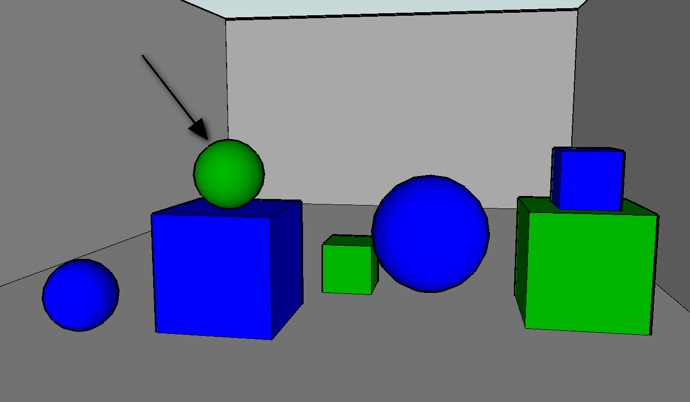
\includegraphics[width=\textwidth]{images/3.jpg}
\caption{Input model}
\label{GRE3D7-stimulus}
\end{minipage}
\hspace{0.5cm}
\begin{minipage}[b]{0.45\linewidth}
\centering
text 
text text text text text text text text text text text text text text text text text text text text text text text text text text text text text text text text text text text text text text text 
\caption{Model as a labeled graph}
\label{GRE3D7-stimulus-graph}
\end{minipage}
\end{figure}



The first thing that we saw is there are algorithms that gives all properties of element before give a relation with another elements, but it see not human. A human can use relations, properties but there is not standard form of use, it mean not everytimes human use properties or relation it depends of the situation. In order to take into account this problem and give more human reference expresion we modify the model for give the same importance to properties and relation, we create a dummy element wich is going to be related to each elements with te relation of the properties that the elements has, it mean every property is going to be a relation with the dummy element ``c'' like we show in the example.

\begin{verbatim}
<problem refer-to="b1">
  <individual id="b1">
    <related rel="yellow" to="c" />
    <related rel="bowl" to="c" />
  </individual>

  <individual id="b2">
    <related rel="red" to="c" />
    <related rel="bowl" to="c" />
  </individual>

  <individual id="b3">
    <related rel="blue" to="c" />
    <related rel="cube" to="c" />
    <related="bellow" to="b1" />
  </individual>
  
  <individual id="c">
  </individual>
</problem>
\end{verbatim}

and plus, we use the probabilities for properties and relation calculated from a human corpora.
With this background we explain the algorithm.

$\REL$ is the set of relation symbols in the signature. It include the properties that are right now relation to the dummy simbol ``c''. 

For each $R \in \REL$ we asume defined two values $R.\puse \in \IR$, the 
probability of using relation $R$ in a RE; and $R.\pdisc \in \IR$, the 
probability that the hearer recognizes relation $R$. 

The algorithm compute the $\mathcal{L}$-similarity sets from a model. 
We are going to have 2 set of formulas, the first one set of formulas are that have not overspecification, and give the limit of iterations of the program, and the second one set of formulas gives overspecification for some elements in case that they run enough for found them.

We calculate two random numbers for each relation, those random numbers are fixed for the entire execution, one for use an another for discernibility. 

it mean that we want not to re-calculate the random in each time for relation, it is like a human don't chance your main of if a word is used or not and if it is discernible or not.

How the algorithm take the goal?
While there is change in the first set os formulas, for each of the relation ordered by higher probability of use, if the probability of use if higher than random probability of the relation for each partition at the moment if the probability of discernibility is higher than the random probability of the relation we add the informatives formulas of each side of set of formulas, but if the discernibility probability of the relation is less than the random probability for that relation we only add the formula to the right side, it is the side that have overspecification.
When no chance of the left side is made the algorithm finish. You can see that sometimes the algorithm generate one overspecification and finish because not see change in the left side, it is to prevent the non-termination of the algorithm.


\begin{algorithm}[h]
\dontprintsemicolon
\caption{Computing the $\mathcal{L}$-similarity sets}\label{algo:bisim-l}
\KwIn{A model $\gM = (\Delta, \interp{\cdot})$ , a list $Rs \in (\REL \times I\!\!R)^*$
 of relation symbols with their \puse values
}
\KwOut{A set of formulas \RE such that
$\{\interp{\varphi} \mid \varphi \in \RE\}$ is the set of
$\mathcal{L}$-similarity 
sets of $\gM$.}

$\RE \leftarrow \{\top\}$

\For{$(R,R.\puse) \in Rs$}{
	$R.\randomuse$ = Random()\\
}
\While{$\exists \varphi \in \RE. |\interp{\varphi_O}|>1$}{
    \RE' $\leftarrow$ \RE \;
    \For{$(R, R.\puse) \in Rs$}{
        \If{$R.\randomuse \le R.\puse$}{
            \For{$\varphi \in \RE$}{
                add$_\mathcal{L}(R, \varphi, \RE)$}
                }\;
            \If{\RE $\not =$ \RE'}{exit}
            }
   \If{\RE $=$ \RE'}{exit}
}
\end{algorithm}

\begin{algorithm}[h]
\dontprintsemicolon
\caption{add$_\el(R, \varphi, \RE)$} \label{algo:bisim-add-el}
\If{$R.\randomdisc \le R.\pdisc$}{
\For{$(\psi_O,\psi_R) \in \RE$ with $|\interp{\psi_O}| > 1$}{
  \If{$\psi_O \sqcap \exists R.\varphi_O$ is not subsumed in $\RE$ {\bf and}
    $\interp{\psi_O \sqcap \exists R.\varphi_O} \neq \emptyset$ {\bf and}
    $\interp{\psi_O \sqcap \exists R.\varphi_O} \neq \interp{\psi_O}$}{
    add $(\psi_O \sqcap \exists R.\varphi_O, \psi_R \sqcap \exists R.\varphi_R)$ to $\RE$ \;
    remove subsumed formulas from $\RE$\;
  }
}
}
\Else{
%\For{$(\psi_O,\psi_R) \in \RE$ with $|\interp{\psi_O}| > 1$}{
%  \If{
%    $\interp{\psi_R \sqcap \exists R.\varphi_R} \neq \emptyset$}
%    {
%    add $(\psi_O, \psi_R \sqcap \exists R.\varphi_R)$ to $\RE$ \;
%    }
\For{$(\psi_O,\psi_R) \in \RE$ with $|\interp{\psi_O}| > 1$}{
  \If{%$\psi_O \sqcap \exists R.\varphi_O$ is not subsumed in $\RE$ {\bf and}
    $\interp{\psi_R \sqcap \exists R.\varphi_R} \neq \emptyset$ {\bf and}
    $\interp{\psi_R \sqcap \exists R.\varphi_R} \neq \interp{\psi_R}$}{
    add $(\psi_O, \psi_R \sqcap \exists R.\varphi_R)$ to $\RE$ \;
    %remove subsumed formulas from $\RE$\; No borramos porque no afectamos a fiO
    }
  }
}
\end{algorithm}

